\prob
{
    Prove that the next matrix is totally unimodular.
    \begin{center}
        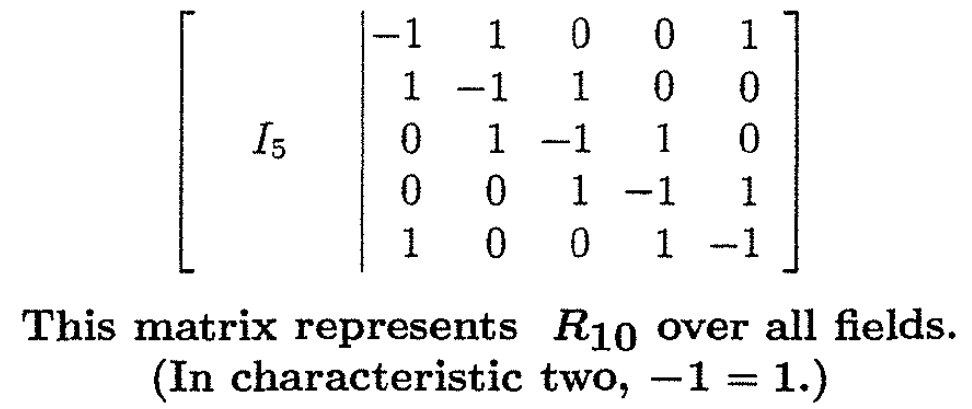
\includegraphics[width=8cm]{Test3/Problem2/R10.png}
    \end{center}\pn
}
\begin{proof}
    As in the previous problem we are going to approach each case.
    
    \begin{itemize}
        \item [case $1 \times 1$]
            Any entrie is -1, 0 or 1, so its determinat will be -1, 0 or 1.\pn
        \item [case $2 \times 2$]
            As we saw before, any column containing only one non-zero entry will result in the determinant of a 
            $1 \times 1$ with a possibly change of sign, and any column with only zeros will result in a determinant
            zero. Then, the only case left is the case with no zero entries.\pn
            
            There is essentially one case, which is
                \begin{align}
                    N =
                        \bordermatrix{
                                &       &       \cr
                                &   1   &  -1   \cr
                                &  -1   &   1  
                        }    
                \end{align}
                
           (given to ones in a column, there is no other column which contains non-zero values in the same rows).
           The determinant of $N$ is 0 and then we have finished this part of the proof.
        
        \item [case $3 \times 3$].
            Suppose we have a submatrix $N$ with a column with two non-zero entries.
        \item [case $4 \times 4$].
        \item [case $5 \times 5$].
    \end{itemize}
\end{proof}